\subsection{Mechanisms of spatial variation}\label{sec:variation}
We compare three treatments of background traffic: absent, fixed at its
baseline link flows, and responsive through endogenous route choice.
Eight largest published OD demands, all incident to node 10, change
jointly from $0.2$ to $1.6$ times their base values; every study OD has
ten fixed paths. The responsive-background assignment assigns all 528
positive demands (full protocols in Appendix~\ref{supp:fields}).
Uniform weights provide a compatible control. The active-link outcome $T(F)=F_{10\to16}$ preserves the $(10,16)$ direction but permits a response-dependent scale; TSTT produces internal imbalance. Figure~\ref{fig:respfield} illustrates the three patterns on the same realized response: compatible weights give one common boundary value on every boundary, the directional outcome balances along the OD but scales with the response, and TSTT weights generate genuine spatial structure. For its seed-zero TSTT response, expanding $\{10\}$ to $\{10,17\}$ lowers the boundary value from $5.77\times10^4$ to $4.34\times10^4$, approximately $92\%$ of the unrestricted spread. The direct-SUE decrease is $24.80\%$ of its own origin-cut value (Appendix~\ref{supp:accuracy}). Both sides of these regions are connected. Free-flow weights explain $84.7\%$ of the node-17 imbalance: all incident links have free-flow time 2 except $10\leftrightarrow17$ with time 8, giving $[B\operatorname{diag}(t_0)g_j]_{17}=6(g_{10\to17,j}-g_{17\to10,j})$.
\begin{figure}[pos=t]
\centering
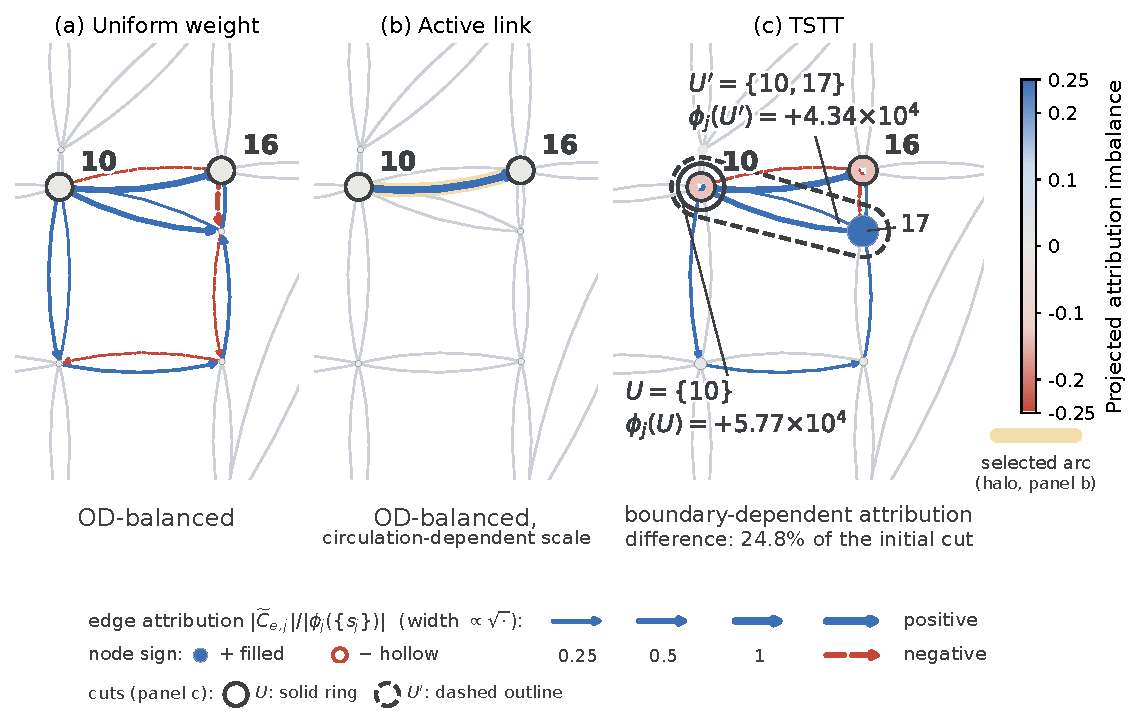
\includegraphics[width=0.9\linewidth]{../figures/fig_resp_field_v109.pdf}
\caption{OD $(10,16)$ endpoint attributions, no-background
assignment, learned
seed $0$. (a) Uniform weights give cut consistency. (b) The signed
TSTT boundary attribution decreases by $24.8\%$ when the boundary expands
from $\{10\}$ to $\{10,17\}$; the active-link outcome --- which
balances in the OD direction but has no response-independent scale ---
is reported in Appendix~\ref{supp:accuracy}. Widths encode attribution
magnitude on the shared square-root scale; node colors show the
projected attribution imbalance $(d_j)_v$ (Eq.~\eqref{eq:endpointd})
divided by the absolute origin-cut value.}
\label{fig:respfield}
\end{figure}

Rerouting produces appreciable spatial variation for every query, and
connected regions retain $60.41$--$76.85\%$ of the unrestricted range
across the full set (complete per-query records for all three
background treatments in Appendix~\ref{supp:additional},
Tables~\ref{tab:bgfull} and~\ref{tab:cutspreadfull}). Normalizations use each setting's own origin boundary value: for
$(17,10)$, the percentage falls from $59.95\%$ under the no-background
treatment to $54.77\%$ under the responsive-background treatment while
the absolute spread rises from 17,607.8 to 123,202.1, approximately
sevenfold.
\paragraph{Response decomposition at common states.}\label{subsec:bgsplit}
Comparing the three background treatments changes both costs and sensitivities. At each common responsive-background state, the mechanism decomposition separates the attribution into study and background response parts, with $BJ_j^{\mathrm{study}}=\mu_j$ and $BJ_j^{\mathrm{bg}}=0$, both weighted by the same total-flow TSTT gradient:
\begin{equation}
c_j^{\mathrm{tot}}=c_j^{\mathrm{study}}+c_j^{\mathrm{bg}}.
\label{eq:bg_attribution}
\end{equation}
At node 15 for $(10,16)$, study and background divergence contributions are $-973.1$ and $49{,}103.4$. Yet on the specified expansion $\{10\}\to\{10,17\}$, the attribution changes only $-3361.1$ ($-1305.0$ study, $-2056.1$ background), or $1.23\%$ of the initial attribution. Large extremal variation can coexist with similar selected boundary values. Component differences add at a fixed region pair; their separate ranges do not add in general.

\paragraph{Free-flow and congestion mechanisms.}\label{subsec:newod}
For BPR costs, $g_e'=t_{0,e}+0.75t_{0,e}(F_e/c_e)^4$. Crossing these two weight terms with the two response terms gives four additive contributions, evaluated at identical states and the same reported boundary:
\[
\phi_j(U_-)=\sum_{a\in\{\mathrm{ff,cong}\}}\sum_{b\in\{\mathrm{study,bg}\}}\phi_j^{a,b},
\qquad \phi_j^{a,b}=-\Delta q_j\int_0^1\mathbf1_{U_-}^{\top}BD_\lambda^aJ_j^b(\lambda)\,d\lambda.
\]
Table~\ref{tab:ffcong} distinguishes the mechanisms behind the sign-crossing queries of Table~\ref{tab:newod}: study congestion dominates $(1,19)$, both congestion terms are negative for $(1,15)$, and background congestion dominates $(7,12)$. The combined free-flow contribution stays positive. The decomposition is additive at a common equilibrium state and identifies the contribution of each response--weight component.
\begin{table}[pos=htbp]
\caption{Four parts of the same boundary attribution at the reported
$U_-$ (responsive-background six-query protocol; TSTT units; identical $41$-point
states, responses, and boundaries as Table~\ref{tab:newod}). Study
includes all six query ODs; background includes the other $522$.
Columns cross free-flow/congestion weights with study/background
responses. Entries are rounded independently.}\label{tab:ffcong}
\small
\begin{tabular*}{\tblwidth}{@{\extracolsep{\fill}}lrrrrr}
\toprule
OD & Free-flow study & Free-flow background & Congestion study & Congestion background & Total\\
\midrule
$(1,19)$ & $-361.3$ & $+759.0$ & $-17{,}357.9$ & $+3{,}458.6$ & $-13{,}501.6$ \\
$(1,15)$ & $+1{,}541.8$ & $+333.8$ & $-6{,}537.4$ & $-3{,}624.2$ & $-8{,}286.0$ \\
$(7,12)$ & $+3{,}897.0$ & $-1{,}311.1$ & $+125.5$ & $-20{,}327.6$ & $-17{,}616.2$ \\
\bottomrule
\end{tabular*}
\end{table}
The sign pattern itself is a spatial property, not a magnitude artifact. Negative attributions occupy $17.8\%$, $2.5\%$ and $7.3\%$ of the 14,477, 15,191 and 16,943 connected regions of the three sign-crossing queries. For $(1,19)$, the connected minimum $-13{,}501.6$ is attained on a 13-node region, whereas a 13-node free-flow neighborhood has attribution $+10{,}756.0$: region size alone does not determine the attribution. At the minimizing boundary, outgoing attributions sum to $7{,}867.3$ and incoming attributions to $21{,}368.8$, so the signed crossing-link attribution is negative while $C_j=50{,}097.7>0$; Figure~\ref{fig:negmech} maps all 26 crossing links. The same contrast appears on the straight screenlines of the prespecified geometric family, whose minimum and maximum attributions for $(1,19)$ have opposite signs under one positive network-wide contribution (Figure~\ref{fig:screenlines}, Appendix~\ref{supp:additional}).
The straight-screenline family uses 36 directions at $5^\circ$ intervals, gaps between node projections, two-sided connectivity and duplicate removal; construction is independent of attribution. It contains 23--152 distinct regions per query. The $(1,19)$ and $(7,12)$ negative minima occur on 2/152 and 10/148 screenlines. Origin-centered hop and free-flow neighborhoods remain positive but can differ in magnitude by factors 8.9, 9.0 and 3.4 for the three sign-crossing queries (Appendix~\ref{supp:newodaccuracy}). Sign stability and common-value accuracy are distinct properties.

\paragraph{Stability under alternative attribution paths.}\label{subsec:pathrobust}
With several ODs changing jointly, the per-query columns depend on the
demand path; twenty-two piecewise-linear alternatives to the
straight-line transition (canonical order, reverse order, twenty
fixed-seed random permutations; identical endpoints, quadrature and
family) leave every spatial conclusion unchanged: system contributions
move by at most $3.4\%$, sign-crossing status is identical on all
orders, common-summary errors shift by at most $0.2$ percentage
points, and the dominant mechanism is unchanged. The profiles are
path-specific in their fine structure (deviations $0.3$--$4.7\%$) but
not in their traffic interpretation; the complete per-order comparison
appears in Table~\ref{tab:pathrobust} (Appendix~\ref{supp:pathrobust}).
